\whiteBGstarBegin
\setcounter{section}{0}
\section{Khúc xạ ánh sáng}
\begin{enumerate}[label=\bfseries Câu \arabic*:]
	
	\item \mkstar{2} 
	
	\cauhoi{
		
		\textbf{(Đề chính thức của BGDĐT - 2018)} Chiết suất của nước và của thủy tinh đối với một ánh sáng đơn sắc có giá trị lần lượt là 1,333 và 1,532. Chiết suất tỉ đối của nước đối với thủy tinh ứng với ánh sáng đơn sắc này là
		\begin{mcq}(4)
			\item 0,199.			
			\item 0,870.			
			\item 1,433.			
			\item 1,149.
		\end{mcq}
	}
	
	\loigiai{
		\textbf{Đáp án: B.}
		
		Chiết suất tỉ đối của nước so với thủy tinh ứng với ánh sáng đơn sắc 
		
		$$ n = \dfrac{\text{1,333}}{\text{1,532}} = \text{0,87}.$$
		
		
		
	}
	
	\item \mkstar{2} 
	
	\cauhoi{
		
		(Đề chính thức của BGDĐT - 2018) Chiếu một tia sáng đơn sắc từ không khí tới mặt nước với góc tới $60^\circ$, tia khúc xạ đi vào trong nước với góc khúc xạ là $r$. Biết chiết suất của không khí và của nước đối với ánh sáng đơn sắc này lần lượt là 1 và 1,333. Giá trị của $r$ là
	\begin{mcq}(4)
	\item $\text{37,97}^\circ$.			
	\item $\text{22,03}^\circ$.			
	\item $\text{40,52}^\circ$.			
	\item $\text{19,48}^\circ$.
	\end{mcq}
		
	}
	
	\loigiai{
		\textbf{Đáp án: C.}
		
		Giá trị của góc khúc xạ r được xác định bởi biểu thức :
		
		$$ \dfrac{\sin i}{\sin r} = n \Rightarrow r = \text{40,52}^\circ.$$
	}
	
	\item \mkstar{2} 
	
	\cauhoi{
		
		Tính tốc độ của ánh sáng trong thủy tinh. Biết thủy tinh có chiết suất $n = \text{1,6}$ và tốc độ ánh sáng trong chân không là $c = 3\cdot 10^8\ \text{m/s}$.
		\begin{mcq}(4)
			\item 2,23$\cdot 10^8\ \text{m/s}$.		
			\item 1,875$\cdot 10^8\ \text{m/s}$. 		
			\item 2,75$\cdot 10^8\ \text{m/s}$.		
			\item 1,5$\cdot 10^8\ \text{m/s}$.
		\end{mcq}
	}
	
	\loigiai{
				
		\textbf{Đáp án: B.}
		
		Tốc độ của ánh sáng trong thủy tinh
		
		$$n = \dfrac{c}{v} \Rightarrow v = \dfrac{c}{n} = \text{1,875} \cdot 10^8\ \text{m/s}.$$
		
	}
	
	
	\item \mkstar{2}
	
	\cauhoi{
		
		Một tia sáng truyền từ môi trường A vào môi trường B dưới góc tới $6^\circ$ thì góc khúc xạ là $8^\circ$. Tính tốc độ ánh sáng trong môi trường A. Biết tốc độ ánh sáng trường môi trường B là 2$\cdot 10^5$ km/s.
		\begin{mcq}(4)
			\item 2,25$\cdot 10^5$ km/s. 		
			\item 2,3$\cdot 10^5$ km/s.		
			\item l,5$\cdot 10^5$ km/s. 		
			\item 2,5$\cdot 10^5$ km/s.
		\end{mcq}
	}
	
	\loigiai{
		
		\textbf{Đáp án: C.}
		
		Ta có:
		
		$$\dfrac{v_1}{v_2} = \dfrac{n_2}{n_1} = \dfrac{\sin i}{\sin r} \Rightarrow v_1 = \text{1,5} \cdot 10^5\ \text{km/s}.$$
	}
	
	\item \mkstar{2}
	
	\cauhoi{
		
		Tia sáng đi từ nước có chiết suất $n_1 = \dfrac{4}{3}$ sang thủy tinh có chiết suất $n_2 = \text{1,5}$ với góc tới $i = 30^\circ$. Góc khúc xạ và góc lệch $D$ tạo bởi tia khúc xạ và tia tới lần lượt là
		\begin{mcq}(4)
			\item $\text{26,4}^\circ$ và  $\text{3,6}^\circ$.	
			\item $\text{50,34}^\circ$ và  $\text{9,7}^\circ$.		
			\item $\text{34,23}^\circ$ và  $\text{4,23}^\circ$.			
			\item $\text{76,98}^\circ$ và  $\text{47}^\circ$.	
		\end{mcq}
	}
	
	\loigiai{
		
		\textbf{Đáp án: A.}
		
		Ta có:
		
		$$n_1 \sin i = n_2 \sin r \Rightarrow \sin r = \dfrac{n_1 \sin i}{n_2} \Rightarrow r = \text{26,39}^\circ.$$
		
		Lại có:
		
		$$D = i -r \approx \text{3,6}^\circ.$$
		
	}
		\item \mkstar{2}
	
	\cauhoi{
		
		Tia sáng truyền trong không khí tới gặp mặt thoáng của chất lỏng có chiết suất $n =\sqrt 3$. Nếu tia phản xạ và tia khúc xạ vuông góc với nhau thì góc tới bằng 
		\begin{mcq}(4)
			\item $30^\circ$.			
			\item $60^\circ$.			
			\item $75^\circ$.		
			\item $45^\circ$.
		\end{mcq}
	}
	\loigiai{
		
		\textbf{Đáp án: B.}
		
		Theo đầu bài, ta có:
		
		$$n_1 =1; n_2 = \sqrt 3.$$
		
		Gọi $i'$ là góc phản xạ, ta có:
		
		$$i' + r = 90^\circ \Rightarrow i + r =90^\circ.$$
		
		Do góc phản xạ bằng góc tới.
		
		Theo định luật khúc xạ ánh sáng, ta có:
		
		$$n_1 \sin i = n_2 \sin r \Rightarrow \tan i = \sqrt 3 \Rightarrow i =60^\circ.$$
		
	}
	\item \mkstar{2}
	
	\cauhoi{
		
		Tia sáng truyền trong không khí tới gặp mặt thoáng của chất lỏng có chiết suất $n = \text{1,6}$. Nếu tia phản xạ và tia khúc xạ hợp với nhau một góc $100^\circ$ thì góc tới bằng
		\begin{mcq}(4)
			\item $36^\circ$.			
			\item $60^\circ$.				
			\item $72^\circ$.				
			\item $51^\circ$.
		\end{mcq}
	}
	\loigiai{
		
		\textbf{Đáp án: D.}
		
		\begin{center}
			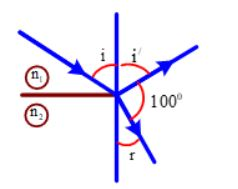
\includegraphics[scale=0.8]{../figs/VN11-2021-PH-TP030-04.JPG}
		\end{center}
	
	Ta có:
	
	$$r = 80^\circ - i .$$
	
	Theo định luật khúc xạ ánh sáng
	
	$$n_1 \sin i = n_2 \sin r \Rightarrow i = \text{50,96}^\circ.$$
	}
	\item \mkstar{3}
	
	\cauhoi{
		
		Một thợ lặn ở dưới nước nhìn thấy Mặt Trời ở độ cao $60^\circ$ so với đường chân trời. Biết chiết suất của nước là $n = \dfrac{4}{3}$. Tính độ cao thực của Mặt Trời so với đường chân trời.
		\begin{mcq}(4)
			\item $38^\circ$.			
			\item $60^\circ$.				
			\item $72^\circ$.				
			\item $48^\circ$.
		\end{mcq}
	}
	\loigiai{
		
		\textbf{Đáp án: D.}
		
		\begin{center}
			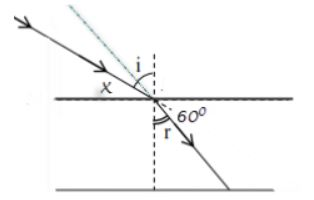
\includegraphics[scale=0.8]{../figs/VN11-2021-PH-TP030-05.JPG}
		\end{center}
	
	Hướng của Mặt Trời mà người thợ lặn nhìn thấy là hướng của các tia sáng khúc xạ vào nước.
	
	$$r = 90^\circ - 60^\circ =30^\circ.$$
	
	Định luật khúc xạ ánh sáng
	
	$$\sin i - n \sin r \Rightarrow i =42^\circ.$$
	
	Độ cao thực của đường chân trời so với mặt trời là 
	
	$$\alpha  = 90^\circ - i  = 48^\circ.$$
		
	}
	\item \mkstar{3}
	
	\cauhoi{
		
		Ba môi trường trong suốt (1), (2), (3) có thể đặt tiếp giáp nhau. Với cùng góc tới $i = 60^\circ$; nếu ánh sáng truyền từ (1) vào (2) thì góc khúc xạ là $45^\circ$; nếu ánh sáng truyền từ (1) vào (3) thì góc khúc xạ là $30^\circ$. Nếu ánh sáng truyền từ (2) vào (3) vẫn với góc tới $i$ thì góc khúc xạ gần giá trị nào nhất sau đây?
		\begin{mcq}(4)
			\item $36^\circ$.			
			\item $60^\circ$.				
			\item $72^\circ$.				
			\item $51^\circ$.
		\end{mcq}
	}
	\loigiai{
		
		\textbf{Đáp án: A.}
		
		Từ (1) đến (2):
		
		$$\dfrac{\sin 60^\circ}{\sin 45^\circ} = \dfrac{n_2}{n_1}$$
		
		Từ (1) đến (3):
		
		$$\dfrac{\sin 60^\circ}{\sin 30^\circ} = \dfrac{n_3}{n_1}$$
		
		Suy ra
		
		$$\dfrac{\sin 45^\circ}{\sin 30^\circ} = \dfrac{n_3}{n_2}$$
		
		Mà từ (2) đến (3):
		
		$$\dfrac{\sin 60^\circ}{\sin r} = \dfrac{n_3}{n_2}$$
		
		Vậy:
		
		$$\dfrac{\sin 45^\circ}{\sin 30^\circ} = \dfrac{\sin 60^\circ}{\sin r} \Rightarrow r =38^\circ.$$
		
		
		
	}



\end{enumerate}

\section{Phản xạ toàn phần}
\begin{enumerate}[label=\bfseries Câu \arabic*:]
	
	\item \mkstar{2} 
	
	\cauhoi{
		
		\textbf{(Đề chính thức của BGD-ĐT - 2018)} Chiếu một tia sáng đơn sắc từ trong nước tới mặt phân cách với không khí. Biết chiết suất của nước và của không khí đối với ánh sáng đơn sắc này lần lượt là 1,333 và 1. Góc giới hạn phản xạ toàn phần ở mặt phân cách giữa nước và không khí đối với ánh sáng đơn sắc này là 
		\begin{mcq}(4)
			\item 41,40$^\circ$.			
			\item 53,12$^\circ$.			
			\item 36,88$^\circ$.			
			\item 48,61$^\circ$.
		\end{mcq}
	}
	
	\loigiai{
		
		\textbf{Đáp án: D.}
		
		Góc giới hạn phản xạ toàn phần ở mặt phân cách giữa nước và không khí đối với ánh sáng đơn sắc này là
		
		$$\sin i_\text{gh} = \dfrac{1}{n} = \text{48,61}^\circ.$$
	}
	
	\item \mkstar{2}
	
	\cauhoi{
		Biết chiết suất của thủy tinh là 1,5 và của nước là $\dfrac{4}{3}$. Góc giới hạn phản xạ toàn phần khi ánh sáng truyền từ thủy tinh sang nước bằng
		\begin{mcq}(4)
			\item 46,8$^\circ$.			
			\item 72,5$^\circ$.			
			\item 62,7$^\circ$.			
			\item 41,8$^\circ$.
		\end{mcq}
	}
	\loigiai{
		
		\textbf{Đáp án: C.}
		
		Góc giới hạn phản xạ toàn phần ở mặt phân cách giữa thủy tinh sang nước đối với ánh sáng đơn sắc này là
		
		$$\sin i_\text{gh} = \dfrac{n_\text{nhỏ}}{n_\text{lớn}}  \Rightarrow i_\text{gh} = \text{62,7}^\circ.$$
	}

		
		\item \mkstar{2}
		
		\cauhoi{
			\begin{minipage}[l]{12cm}
				Một chùm tia sáng hẹp SI truyền trong mặt phẳng tiêt diện vuông góc của một khối trong suốt, đặt trong không khí, tam giác ABC vuông tại A với $\text{AB} = \text{1,2}\ \text{AC}$ như hình vẽ. Tia sáng phản xạ toàn phần ở mặt AC. Trong điều kiện đó, chiết suất n của khối trong suốt có giá trị như thế nào?
			\end{minipage}
			\begin{minipage}[r]{5cm}
				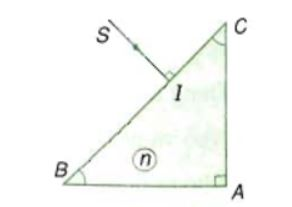
\includegraphics[scale=0.6]{../figs/VN11-PH-35-P-023-1-1.JPG}
			\end{minipage}
				
			\begin{mcq}(4)
				\item $n > \text{1,4}$.				
				\item $n < \text{1,41}$.
				\item $1 < n < \text{1,42}$.			
				\item $n > \text{1,3}$.
			\end{mcq}
		}
		\loigiai{
			
			\textbf{Đáp án: A.}
			
			Tam giác ABC vuông cân tại A.
			
			\begin{center}
				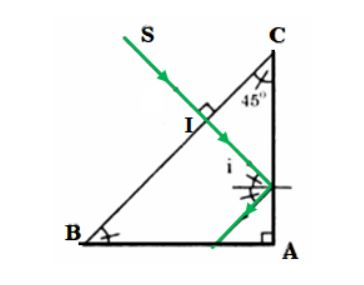
\includegraphics[scale=0.6]{../figs/VN11-2021-PH-TP030-02.JPG}
			\end{center}
			
			Góc B và góc C bằng $45^\circ.$
			
			Mà SI vuông góc BC. Tia sáng SI truyền thẳng vào môi trường trong suốt ABC mà không bị khúc xạ góc tới $i$ ở mặt phẳng BC:
			
			$$ i = 45^\circ \sin i = \sin 45^\circ = \dfrac{1}{\sqrt 2} $$
			
			
			Tia sáng phản xạ toàn phần ở mặt AC 
			
			$$\Rightarrow i \geq i_\text{gh} \Rightarrow \sin i \geq \sin i_\text{gh} = \dfrac{1}{n} \Rightarrow n \geq \sqrt 2.$$
			
			
		}
			\item \mkstar{3}
		
		\cauhoi{
			\begin{minipage}[l]{11cm}
				Một sợi quang hình trụ, lõi có chiết suất $n_1 = \text{1,50}$. Phần vỏ bọc có chiết suất $n_2 = \text{1,414}$. Chùm tia đi từ không khí tới hội tụ ở mặt trước của sợi với góc $2\alpha$ như hình vẽ. Giá trị lớn nhất của $\alpha$ để các tia sáng của chùm truyền đi được trong lõi gần giá trị nào nhất sau đây?
			\end{minipage}
			\begin{minipage}[r]{5cm}
				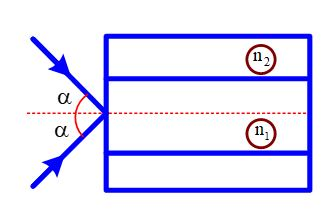
\includegraphics[scale=0.6]{../figs/VN11-PH-35-P-023-1-2.JPG}
			\end{minipage}		
			
			\begin{mcq}(4)
				\item 26$^\circ$.		
				\item 60$^\circ$.			
				\item 30$^\circ$.			
				\item 41$^\circ$.
			\end{mcq}
		}
		\loigiai{
			
			\textbf{Đáp án: C.}
			
			Điều kiện mọi tia sáng trong chùm đều truyền đi được trong ống là phải thỏa mãn điều kiện phản xạ toàn phần tại mặt phân cách của lõi trụ với vỏ bóc của nó.
			
			\begin{center}
				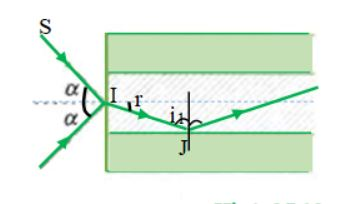
\includegraphics[scale=0.6]{../figs/VN11-2021-PH-TP030-01.JPG}
			\end{center}
		
			Điều kiện phản xạ toàn phần tại J là
			
			$$ i_1 \geq i_\text{gh} \Rightarrow \sin i_1 \geq \sin i_\text{gh} = \dfrac{n_2}{n_1}.$$
			
			Mặt khác:
			
			$$r=90^\circ - i_1 \Rightarrow \cos r = \sin i_1 \geq \dfrac{n_2}{n_1}.$$
			
			Áp dụng định luật khúc xạ tại mặt trước của ống quang ta được:
			
			$$\sin \alpha = n_1 \sin r = n_1 \sqrt{1- \cos^2 r} \leq n_1 \sqrt{1- \left(\dfrac{n_2}{n_1}\right)^2} \Rightarrow \alpha \leq 30^\circ.$$
		}
			\item \mkstar{3}
		
		\cauhoi{
			
			Một cái đinh được cắm vuông góc vào tâm O một tâm gỗ hình tròn có bán kính $R = 5\ \text{cm}$. Tấm gỗ được thả nổi trên mặt thoáng của một chậu nước. Đầu A của đỉnh trong nước. Cho chiết suất của nước là $n = \dfrac{4}{3}$. Để mắt không còn nhìn thấy đầu A của đỉnh thì khoảng cách OA lớn nhất là
			\begin{mcq}(4)
				\item 6,5 cm.			
				\item 7,2 cm.			
				\item 4,4 cm.			
				\item 5,6 cm.
			\end{mcq}
		}
		\loigiai{
			
			\textbf{Đáp án: C.}
			
			\begin{center}
				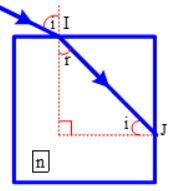
\includegraphics[scale=0.8]{../figs/VN11-2021-PH-TP030-03.JPG}
			\end{center}
		
		$$\dfrac{\sin i}{\sin r} = \dfrac{n_2}{n_1} \Rightarrow i = \text{48,59}^\circ.$$
		
		$$\text{OA} = \dfrac{\text{OI}}{\tan r} = \text{4,41}\ \text{cm}.$$
		}
		
\end{enumerate}
\whiteBGstarEnd